\documentclass[a4paper,10pt]{article}
%\documentclass[a4paper,10pt]{scrartcl}

\usepackage[utf8]{inputenc}
\usepackage{pgf}
\usepackage{tikz}
\usepackage{float}
\usepackage{stmaryrd}
\usetikzlibrary{arrows}
\usetikzlibrary{automata}
\definecolor{lgrey}{RGB}{190,190,190}
\pdfinfo{%
  /Title    (Assessed Coursework: Systems Verification 303)
  /Author   (Ioannis Kassinopoulos)
  /Creator  (Ioannis Kassinopoulos)
  /Producer (Ioannis Kassinopoulos)
  /Subject  (Systems Verification Coursework)
  /Keywords (verification,coursework,imperial)
}

\begin{document}

\title{Assessed Coursework: Systems Verification}
\author{Ioannis Kassinopoulos}
\date{\today}
\maketitle
\section*{Question 1}
\begin{figure}[H]
  \centering
  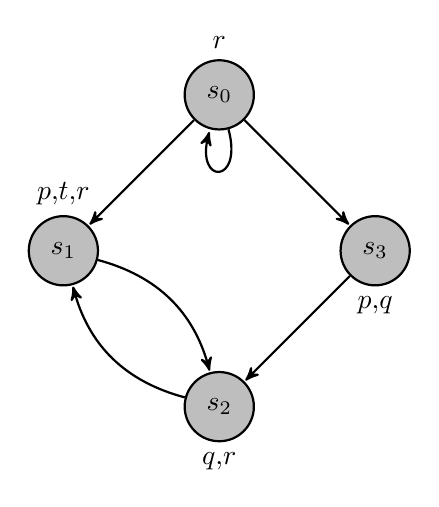
\begin{tikzpicture}[->,>=stealth',shorten >=0.5pt,auto,node distance=2.8cm,thick]
      \tikzstyle{every state}=[fill=lgrey,draw=black,text=black]

      \node[label = above:{$r$},state]		(A) {$s_0$};
      \node[label = above:{$p$,$t$,$r$},state]	(B) [below left of  = A]   {$s_1$};
      \node[label = below:{$p$,$q$},state]	(C) [below right of = A]   {$s_3$};
      \node[label = below:{$q$,$r$},state]	(D) [below right of = B]   {$s_2$};
      
      \path 
	(A) edge			node{} (B)
	(A) edge			node{} (C)
	(A) edge	[loop below]	node{} (A)
	(B) edge	[bend left]	node{} (D)
	(D) edge	[bend left]	node{} (B)
	(C) edge			node{} (D);
      
  \end{tikzpicture}
  \caption{The transition system $\mathcal{M}_1$.}
  \label{fig:m1}
\end{figure}

\subsection*{Algebraic Form}

A transition system $\mathcal{M}=(S,\rightarrow,\pi)$ is a set of states $S$ endowed with a transition relation 
$\rightarrow$ (a binary relation on $S$), such that every $s \in  S$ has some $s'\in S$ with $s\rightarrow s'$,
and an inverse labeling function $\pi:\mathcal{P}\rightarrow S$.
\\[0.5cm] 
Our system $\mathcal{M}_1$ (figure:~\ref{fig:m1}) can be described as following:
\\[0.cm] 
$\mathcal{P} = \{p,q,r,t\}$
\\[0.10cm] 
$\mathcal{M}_1 = \{\{ s_0,s_1,s_2,s_3 \} , \{ (s_0,s_0),(s_0,s_1),(s_0,s_3),(s_1,s_2),(s_2,s_1),(s_3,s_1)   \} , \pi \}$
\\[0.10cm] 
$\pi(p) = \{s_1,s_3 \}$
\\[0.10cm] 
$\pi(q) = \{s_2,s_3 \}$
\\[0.10cm] 
$\pi(r) = \{s_0,s_1,s_2 \}$
\\[0.10cm] 
$\pi(t) = \{ s_1 \}$
\subsection*{Infinite Tree}
\begin{figure}[H]
  \label{fig:infTree}
  \centering
  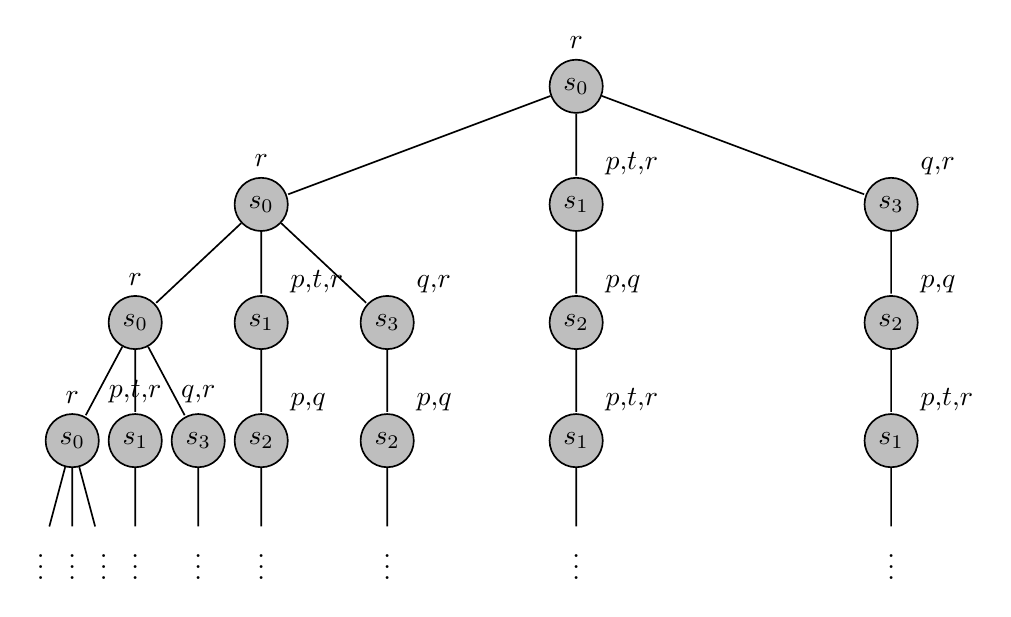
\begin{tikzpicture}[level 2/.style={sibling distance=16mm},level 1/.style={sibling distance=40mm},level 4/.style={sibling distance=4mm},level 3/.style={sibling distance=8mm},level/.style={sibling distance=25mm/#1},-,>=stealth',shorten >=0.5pt,auto,node distance=1cm,semithick]
      \tikzstyle{every state}=[fill=lgrey,draw=black,text=black,inner sep=3pt,minimum size=4pt]
      \node [label = above:{$r$},state] (a){$s_0$}
	child {
	node [label = above:{$r$},state] (b) {$s_0$}
	  child {
	  node [label = above:{$r$},state] (c) {$s_0$}
	    child{
	    node [label = above:{$r$},state] (d) {$s_0$}
	      child{
	      node [] (e) {$\vdots$}
	      }
	      child{
	      node [] (e) {$\vdots$}
	      }
	      child{
	      node [] (e) {$\vdots$}
	      }
	    }
	    child{
	    node [label = above:{$p$,$t$,$r$},state] (d) {$s_1$}
	      child{
	      node [] (e) {$\vdots$}
	      }
	    }
	    child{
	    node [label = above:{$q$,$r$},state] (d) {$s_3$}
	    child{
	      node [] (e) {$\vdots$}
	      }
	    }
	  }
	  child {
	  node [label = above right:{$p$,$t$,$r$},state] (c) {$s_1$}
	    child {
	    node [label = above right:{$p$,$q$},state] (d) {$s_2$}	      
	    child {
	    node [] (e) {$\vdots$}	      
	    }
	    }
	  }	  
	  child {
	    node [label = above right:{$q$,$r$},state] (c) {$s_3$}
	      child {
	      node [label = above right:{$p$,$q$},state] (d) {$s_2$}	      
		child {
		node [] (e) {$\vdots$}	      
	      }
	    }
	  }
	}
	child {
	node [label = above right:{$p$,$t$,$r$},state] (b) {$s_1$}
	  child {
	  node [label = above right:{$p$,$q$},state] (c) {$s_2$}
	    child {
	    node [label = above right:{$p$,$t$,$r$},state] (d) {$s_1$}
	      child {
	      node [] (e) {$\vdots$}	      
	      }
	    }
	  }
	}
	child {
	node [label = above right:{$q$,$r$},state] (b) {$s_3$}
	child {
	node [label = above right:{$p$,$q$},state] (c) {$s_2$}
	  child {
	  node [label = above right:{$p$,$t$,$r$},state] (d) {$s_1$}
	    child {
	    node [] (e) {$\vdots$}
	    }
	  }
	}
	};
  \end{tikzpicture}
  \caption{Unwinding the system described by  $\mathcal{M}_1$ as an infinite tree of all computation paths beginning in $s_0$ (first layer).}
\end{figure}

\subsection*{Satisfiability}

\newpage
\section*{Question 2}
\begin{figure}[H]
  \centering
  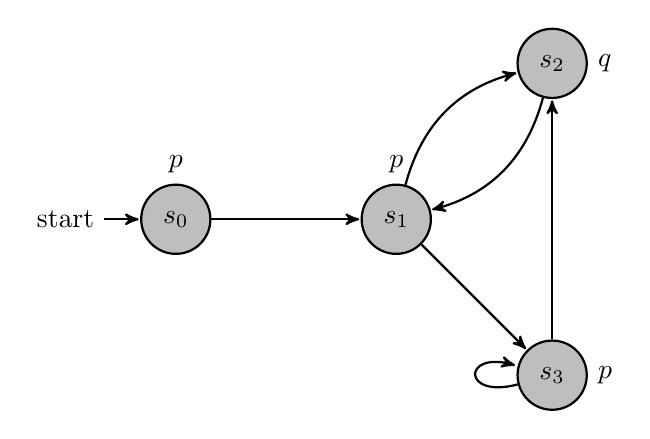
\begin{tikzpicture}[->,>=stealth',shorten >=0.5pt,auto,node distance=2.8cm,thick]
      \tikzstyle{every state}=[fill=lgrey,draw=black,text=black]

      \node[label = above:{$p$},initial,state]		(A) {$s_0$};
      \node[label = above:{$p$},state]		(B) [right of = A] {$s_1$};
      \node[label = right:{$q$},state]		(C) [above right of = B] {$s_2$};
      \node[label = right:{$p$},state]		(D) [below right of = B] {$s_3$};
      
      \path 
	(A) edge			node{} (B)
	(B) edge	[bend left]	node{} (C)
	(C) edge	[bend left]	node{} (B)
	(B) edge			node{} (D)
	(D) edge			node{} (C)
	(D) edge	[loop left]	node{} (D);
  \end{tikzpicture}
  \caption{The transition system $\mathcal{M}_2$.}
  \label{fig:m2}
\end{figure}

\subsection*{Calculating}

\subsection*{$\phi = p$}
\hspace*{5mm} $SAT(p)=\{ s \in S \mid p\in L(s)\} = \{s_0,s_1,s_2\}$ 
\\[0.25cm] 
\hspace*{5mm} $\Rightarrow \llbracket \phi \rrbracket = \{s_0,s_1,s_2\}$
\subsection*{$\phi = AGEFp$}
\hspace*{5mm} $SAT(EFp)=SAT(E[trueUp])=SAT_{eu}(true,p)$ 
\\[0.25cm] 
\hspace*{5mm}$SAT_{eu}(true,p)$ 
\\[0.25cm] 
\hspace*{10mm} $W = \{s_0,s_1,s_2,s_3\}$ 
\\[0.25cm] 
\hspace*{10mm} $Y_0 = \{s_0,s_1,s_3\}$ 
\\[0.25cm] 
\hspace*{10mm} $Y_1 = \{s_0,s_1,s_2,s_3\}$ 
\\[0.25cm] 
\hspace*{10mm} $Y_2 = Y_1$ 
\\[0.25cm] 
\hspace*{5mm} $SAT(AGEFp)=SAT(\neg EF \neg EF p)$ 
\\[0.25cm] 
\hspace*{5mm} $SAT(EF \neg EF p) =  SAT(E[trueU\neg EF p]) = SAT_{eu}(true,\neg EF p)$ 
\\[0.25cm] 
\hspace*{5mm} $SAT_{eu}(true,\neg EF p)$ 
\\[0.25cm] 
\hspace*{10mm} $W = \{s_0,s_1,s_2,s_3\}$ 
\\[0.25cm] 
\hspace*{10mm} $Y_0 = S \backslash \{s_0,s_1,s_2,s_3\} = \{ \}$ 
\\[0.25cm] 
\hspace*{10mm} $Y_1 = Y_0$ 
\\[0.25cm] 
\hspace*{4.9mm} $SAT(AGEFp)=SAT(\neg EF \neg EF p) = S\backslash SAT(EF \neg EF p) = \{s_0,s_1,s_2,s_3 \}$ 
\\[0.25cm] 
\hspace*{5mm} $\Rightarrow \llbracket \phi \rrbracket = \{s_0,s_1,s_2,s_3\}$

\subsection*{$\phi = AFq$}
\hspace*{5mm}$SAT(AFq) = SAT_{af}(q)$ 
\\[0.25cm] 
\hspace*{5mm}$Y_0 = \{s_2\}$
\\[0.25cm] 
\hspace*{5mm}$Y_1 = Y_0$ 
\\[0.25cm] 
\hspace*{5mm} $\Rightarrow \llbracket \phi \rrbracket = \{s_2\}$


\subsection*{$\phi = AGp \vee Afq$}
\subsection*{$\phi = E(pU(AFq))$}






\newpage
\section*{Question 3}
\newpage
\section*{Question 4}
Let $\phi = (x_1 \wedge x_2) \vee (y_1 \wedge y_2) $, the following truth table is derived to help us with our calculations

\begin{center}
 
\begin{tabular}{|c|c|c|c|c|c|c|}
\hline
$x_1$ & $x_2$ & $y_1$ & $y_2$ & $x_1 \wedge x_2 $ & $y_1 \wedge y_2$ & $(x_1 \wedge x_2) \vee (y_1 \wedge y_2)$ \\
\hline
0 & 0 & 0 & 0 & 0 & 0 & 0 \\
0 & 0 & 0 & 1 & 0 & 0 & 0 \\
0 & 0 & 1 & 0 & 0 & 0 & 0 \\
0 & 0 & 1 & 1 & 0 & 1 & 1 \\
0 & 1 & 0 & 0 & 0 & 0 & 0 \\
0 & 1 & 0 & 1 & 0 & 0 & 0 \\
0 & 1 & 1 & 0 & 0 & 0 & 0 \\
0 & 1 & 1 & 1 & 0 & 1 & 1 \\
1 & 0 & 0 & 0 & 0 & 0 & 0 \\
1 & 0 & 0 & 1 & 0 & 0 & 0 \\
1 & 0 & 1 & 0 & 0 & 0 & 0 \\
1 & 0 & 1 & 1 & 0 & 1 & 1 \\
1 & 1 & 0 & 0 & 1 & 0 & 1 \\
1 & 1 & 0 & 1 & 1 & 0 & 1 \\
1 & 1 & 1 & 0 & 1 & 0 & 1 \\
1 & 1 & 1 & 1 & 1 & 1 & 1 \\

\hline
\end{tabular}

\end{center}

\subsection*{Binary Decision Tree}
\begin{figure}[H]
  \label{fig:bdt}
  \centering
  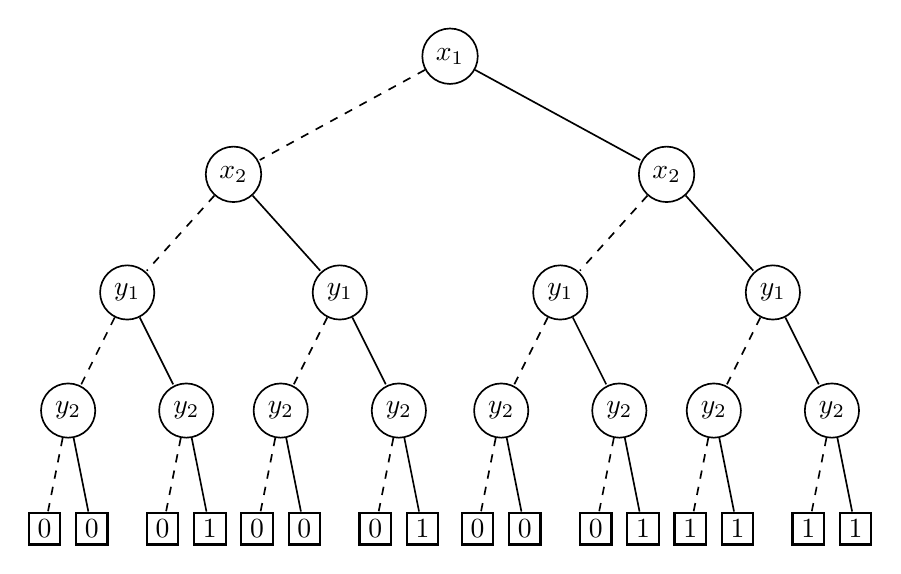
\begin{tikzpicture}[
  level 1/.style={sibling distance=55mm},
  level 2/.style={sibling distance=27mm},
  level 3/.style={sibling distance=15mm},
  level 4/.style={sibling distance=6mm},
  -,>=stealth',shorten >=0.5pt,auto,node distance=1cm,semithick,term/.style={draw,rectangle,minimum size=4mm,inner sep=0pt,outer sep=0pt,solid,thick}]
      \tikzstyle{every state}=[fill=white,draw=black,text=black,inner sep=3pt,minimum size=4pt,solid]
      
      
     \node [state] (a){$x_1$}
     child[dashed]{
      node [state] (b){$x_2$}
      child[dashed]{
	node [state] (c){$y_1$}
	child[dashed]{
	  node [state] (d){$y_2$}
	  child[dashed]{
	    node [term] (e){$0$}	    
	  }
	  child[solid]{
	    node [term] (e){$0$}	    
	  }
	}
	child[solid]{
	  node [state] (d){$y_2$}
	  child[dashed]{
	    node [term] (e){$0$}	    
	  }
	  child[solid]{
	    node [term] (e){$1$}	    
	  }
	}
      }
      child[solid]{
	node [state] (c){$y_1$}
	child[dashed]{
	  node [state] (d){$y_2$}
	  child[dashed]{
	    node [term] (e){$0$}	    
	  }
	  child[solid]{
	    node [term] (e){$0$}	    
	  }
	}
	child[solid]{
	  node [state] (d){$y_2$}
	  child[dashed]{
	    node [term] (e){$0$}	    
	  }
	  child[solid]{
	    node [term] (e){$1$}	    
	  }
	}
      }
     }
     child[solid]{
      node [state] (b){$x_2$}
      child[dashed]{
	node [state] (c){$y_1$}
	child[dashed]{
	  node [state] (d){$y_2$}
	  child[dashed]{
	    node [term] (e){$0$}	    
	  }
	  child[solid]{
	    node [term] (e){$0$}	    
	  }
	}
	child[solid]{
	  node [state] (d){$y_2$}
	  child[dashed]{
	    node [term] (e){$0$}	    
	  }
	  child[solid]{
	    node [term] (e){$1$}	    
	  }
	}
      }
      child[solid]{
	node [state] (c){$y_1$}
	child[dashed]{
	  node [state] (d){$y_2$}
	  child[dashed]{
	    node [term] (e){$1$}	    
	  }
	  child[solid]{
	    node [term] (e){$1$}	    
	  }
	}
	child[solid]{
	  node [state] (d){$y_2$}
	  child[dashed]{
	    node [term] (e){$1$}	    
	  }
	  child[solid]{
	    node [term] (e){$1$}	    
	  }
	}
      }
     };
 
  \end{tikzpicture}
  \caption{A BDT is easily derived from the truth table. Every non-terminal node is labelled with a variable and every terminal node is labelled with either 0 or 1.}
\end{figure}

\subsection*{Reduced Ordered Binary Decision Diagrams}
In order to reduce the size of the BDT we can produce a 
Binary Decision Diagram which is a reduced form of the BDT.
Making this diagram ordered over a list of variables, results in getting an Ordered Binary Decision Diagram (OBDD) which is
then unique when it is reduced until no more reduction can occur. This reduced form is called canonical form and it can be used to
extract equivalences since two different but equivalent Boolean functions always have identically structured Reduced Ordered Binary Decision Diagrams 
if they have compatible variable orderings.
\subsubsection*{Reduction Algorithm}
\noindent In order to reduce BDTs we use iteratively the rules C1-C3 until no more reductions can occur.

\begin{itemize}
\item {\bf C1:} Removal of duplicate terminals. 
\item {\bf C2:} Removal of redundant tests. 
\item {\bf C3:} Removal of duplicate non-terminals. 
\end{itemize}




\subsubsection*{ROBDD under the $[x_1,x_2,y_1,y_2]$ ordering.}

\begin{figure}[H]
  \label{fig:robdd11}
  \centering
  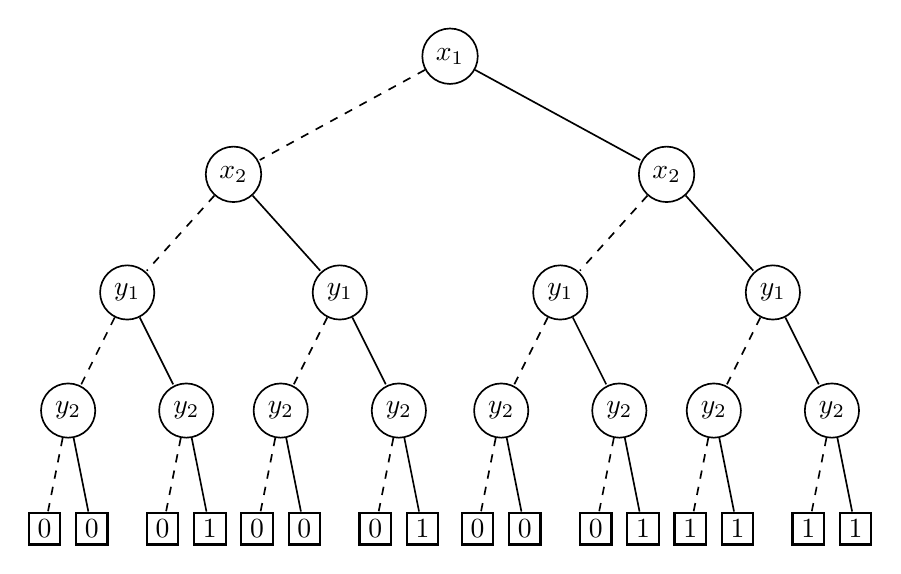
\begin{tikzpicture}[
  level 1/.style={sibling distance=55mm},
  level 2/.style={sibling distance=27mm},
  level 3/.style={sibling distance=15mm},
  level 4/.style={sibling distance=6mm},
  -,>=stealth',shorten >=0.5pt,auto,node distance=1cm,semithick,term/.style={draw,rectangle,minimum size=4mm,inner sep=0pt,outer sep=0pt,solid,thick}]
      \tikzstyle{every state}=[fill=white,draw=black,text=black,inner sep=3pt,minimum size=4pt,solid]
      
      
     \node [state] (a){$x_1$}
     child[dashed]{
      node [state] (b){$x_2$}
      child[dashed]{
	node [state] (c){$y_1$}
	child[dashed]{
	  node [state] (d){$y_2$}
	  child[dashed]{
	    node [term] (e){$0$}	    
	  }
	  child[solid]{
	    node [term] (e){$0$}	    
	  }
	}
	child[solid]{
	  node [state] (d){$y_2$}
	  child[dashed]{
	    node [term] (e){$0$}	    
	  }
	  child[solid]{
	    node [term] (e){$1$}	    
	  }
	}
      }
      child[solid]{
	node [state] (c){$y_1$}
	child[dashed]{
	  node [state] (d){$y_2$}
	  child[dashed]{
	    node [term] (e){$0$}	    
	  }
	  child[solid]{
	    node [term] (e){$0$}	    
	  }
	}
	child[solid]{
	  node [state] (d){$y_2$}
	  child[dashed]{
	    node [term] (e){$0$}	    
	  }
	  child[solid]{
	    node [term] (e){$1$}	    
	  }
	}
      }
     }
     child[solid]{
      node [state] (b){$x_2$}
      child[dashed]{
	node [state] (c){$y_1$}
	child[dashed]{
	  node [state] (d){$y_2$}
	  child[dashed]{
	    node [term] (e){$0$}	    
	  }
	  child[solid]{
	    node [term] (e){$0$}	    
	  }
	}
	child[solid]{
	  node [state] (d){$y_2$}
	  child[dashed]{
	    node [term] (e){$0$}	    
	  }
	  child[solid]{
	    node [term] (e){$1$}	    
	  }
	}
      }
      child[solid]{
	node [state] (c){$y_1$}
	child[dashed]{
	  node [state] (d){$y_2$}
	  child[dashed]{
	    node [term] (e){$1$}	    
	  }
	  child[solid]{
	    node [term] (e){$1$}	    
	  }
	}
	child[solid]{
	  node [state] (d){$y_2$}
	  child[dashed]{
	    node [term] (e){$1$}	    
	  }
	  child[solid]{
	    node [term] (e){$1$}	    
	  }
	}
      }
     };
 
  \end{tikzpicture}
  \caption{We start with the BDT over our ordering.}
\end{figure}


\begin{figure}[H]
  \label{fig:robdd12}
  \centering
  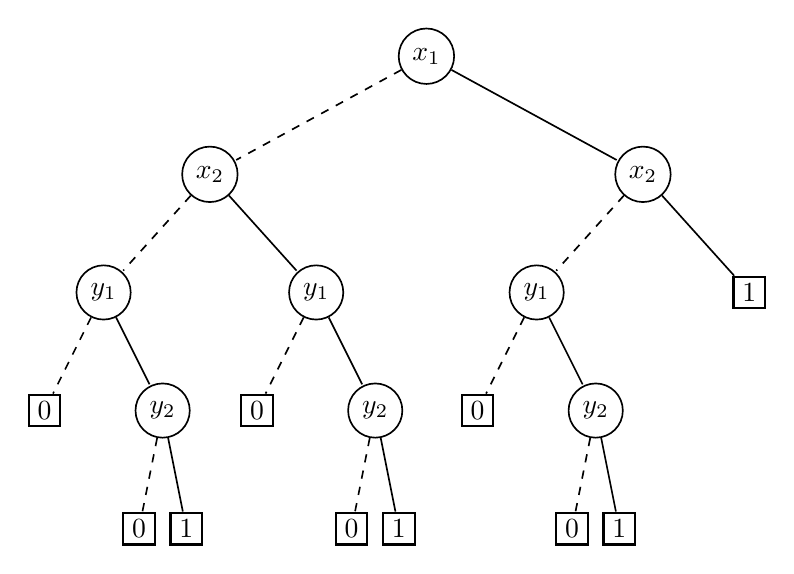
\begin{tikzpicture}[
  level 1/.style={sibling distance=55mm},
  level 2/.style={sibling distance=27mm},
  level 3/.style={sibling distance=15mm},
  level 4/.style={sibling distance=6mm},
  -,>=stealth',shorten >=0.5pt,auto,node distance=1cm,semithick,term/.style={draw,rectangle,minimum size=4mm,inner sep=0pt,outer sep=0pt,solid,thick}]
      \tikzstyle{every state}=[fill=white,draw=black,text=black,inner sep=3pt,minimum size=4pt,solid]
      
      
     \node [state] (a){$x_1$}
     child[dashed]{
      node [state] (b){$x_2$}
      child[dashed]{
	node [state] (c){$y_1$}
	child[dashed]{
	  node [term] (d){$0$}
	}
	child[solid]{
	  node [state] (d){$y_2$}
	  child[dashed]{
	    node [term] (e){$0$}	    
	  }
	  child[solid]{
	    node [term] (e){$1$}	    
	  }
	}
      }
      child[solid]{
	node [state] (c){$y_1$}
	child[dashed]{
	  node [term] (d){$0$}
	 }
	child[solid]{
	  node [state] (d){$y_2$}
	  child[dashed]{
	    node [term] (e){$0$}	    
	  }
	  child[solid]{
	    node [term] (e){$1$}	    
	  }
	}
      }
     }
     child[solid]{
      node [state] (b){$x_2$}
      child[dashed]{
	node [state] (c){$y_1$}
	child[dashed]{
	  node [term] (d){$0$}	  
	}
	child[solid]{
	  node [state] (d){$y_2$}
	  child[dashed]{
	    node [term] (e){$0$}	    
	  }
	  child[solid]{
	    node [term] (e){$1$}	    
	  }
	}
      }
      child[solid]{
	node [term] (c){$1$}
      }
     };
 
  \end{tikzpicture}
  \caption{Using C2 we remove the redundant tests and eliminate the nodes leading to them. We derive the above reduced diagram.}
\end{figure}


\begin{figure}[H]
  \label{fig:robdd1}
  \centering
  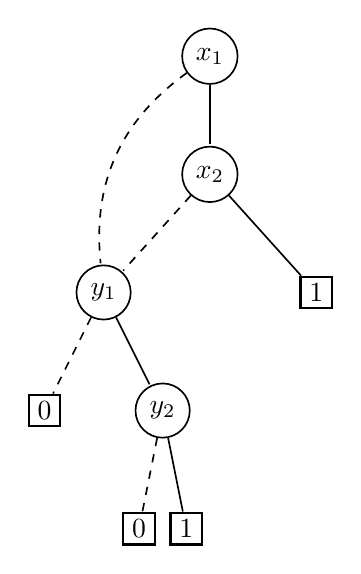
\begin{tikzpicture}[
  level 1/.style={sibling distance=55mm},
  level 2/.style={sibling distance=27mm},
  level 3/.style={sibling distance=15mm},
  level 4/.style={sibling distance=6mm},
  -,>=stealth',shorten >=0.5pt,auto,node distance=1cm,semithick,term/.style={draw,rectangle,minimum size=4mm,inner sep=0pt,outer sep=0pt,solid,thick}]
      \tikzstyle{every state}=[fill=white,draw=black,text=black,inner sep=3pt,minimum size=4pt,solid]
      
      
     \node [state] (A){$x_1$}
     
     child[solid]{
      node [state] (B){$x_2$}
      child[dashed]{
	node [state] (C1){$y_1$}
	child[dashed]{
	  node [term] (D1){$0$}	  
	}
	child[solid]{
	  node [state] (D2){$y_2$}
	  child[dashed]{
	    node [term] (E1){$0$}	    
	  }
	  child[solid]{
	    node [term] (E2){$1$}	    
	  }
	}
      }
      child[solid]{
	node [term] (C2){$1$}
      }
     };
     
     \path 
	(A) edge[dashed,bend right]			node{} (C1);
	
 
  \end{tikzpicture}
  \caption{Using C3 we remove the duplicate non-terminals, redirect the incoming edges and derive the above reduced diagram.}
\end{figure}


\begin{figure}[H]
  \label{fig:robdd13}
  \centering
  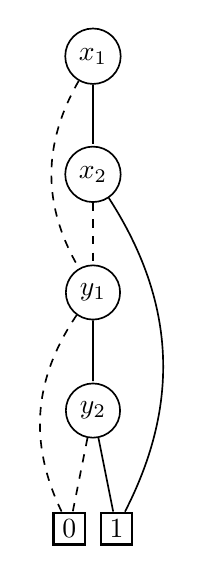
\begin{tikzpicture}[
  level 1/.style={sibling distance=55mm},
  level 2/.style={sibling distance=27mm},
  level 3/.style={sibling distance=15mm},
  level 4/.style={sibling distance=6mm},
  -,>=stealth',shorten >=0.5pt,auto,node distance=1cm,semithick,term/.style={draw,rectangle,minimum size=4mm,inner sep=0pt,outer sep=0pt,solid,thick}]
      \tikzstyle{every state}=[fill=white,draw=black,text=black,inner sep=3pt,minimum size=4pt,solid]
      
      
     \node [state] (A){$x_1$}
     
     child[solid]{
      node [state] (B){$x_2$}
      child[dashed]{
	node [state] (C1){$y_1$}
	child[solid]{
	  node [state] (D2){$y_2$}
	  child[dashed]{
	    node [term] (E1){$0$}	    
	  }
	  child[solid]{
	    node [term] (E2){$1$}	    
	  }
	}
      }
     };
     
     \path 
	(A) edge[dashed,bend right]			node{} (C1)
	(B) edge[bend left]			node{} (E2)
	(C1) edge[dashed,bend right]			node{} (E1);

 
  \end{tikzpicture}
  \caption{Using C1 we remove all the duplicate terminals. This OBDD cannot be reduced any further so we can now call it the canonical of the previous diagrams.}
\end{figure}

\subsubsection*{ROBDD under the $[x_1,y_1,y_2,x_2]$ ordering.}

\begin{figure}[H]
  \label{fig:robdd21}
  \centering
  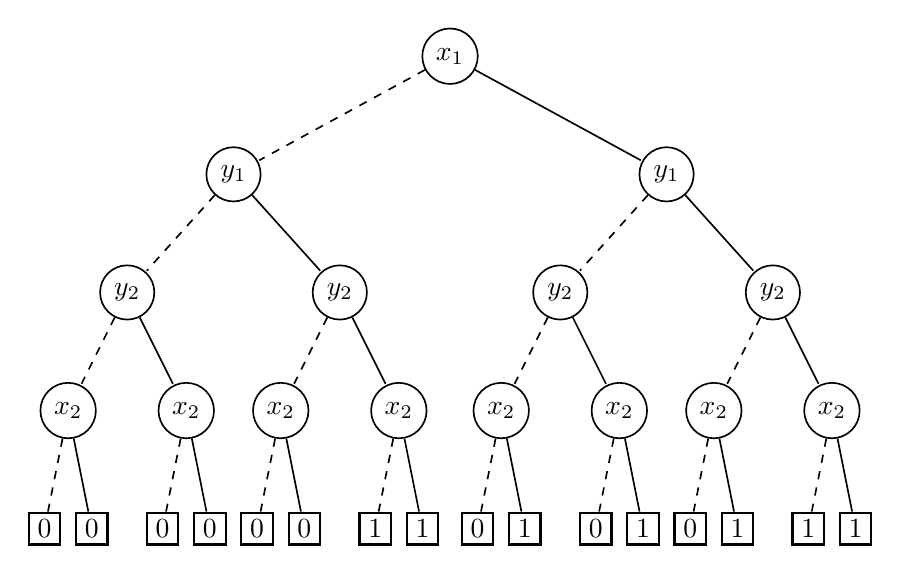
\begin{tikzpicture}[
  level 1/.style={sibling distance=55mm},
  level 2/.style={sibling distance=27mm},
  level 3/.style={sibling distance=15mm},
  level 4/.style={sibling distance=6mm},
  -,>=stealth',shorten >=0.5pt,auto,node distance=1cm,semithick,term/.style={draw,rectangle,minimum size=4mm,inner sep=0pt,outer sep=0pt,solid,thick}]
      \tikzstyle{every state}=[fill=white,draw=black,text=black,inner sep=3pt,minimum size=4pt,solid]
      
      
     \node [state] (a){$x_1$}
     child[dashed]{
      node [state] (b){$y_1$}
      child[dashed]{
	node [state] (c){$y_2$}
	child[dashed]{
	  node [state] (d){$x_2$}
	  child[dashed]{
	    node [term] (e){$0$}	    
	  }
	  child[solid]{
	    node [term] (e){$0$}	    
	  }
	}
	child[solid]{
	  node [state] (d){$x_2$}
	  child[dashed]{
	    node [term] (e){$0$}	    
	  }
	  child[solid]{
	    node [term] (e){$0$}	    
	  }
	}
      }
      child[solid]{
	node [state] (c){$y_2$}
	child[dashed]{
	  node [state] (d){$x_2$}
	  child[dashed]{
	    node [term] (e){$0$}	    
	  }
	  child[solid]{
	    node [term] (e){$0$}	    
	  }
	}
	child[solid]{
	  node [state] (d){$x_2$}
	  child[dashed]{
	    node [term] (e){$1$}	    
	  }
	  child[solid]{
	    node [term] (e){$1$}	    
	  }
	}
      }
     }
     child[solid]{
      node [state] (b){$y_1$}
      child[dashed]{
	node [state] (c){$y_2$}
	child[dashed]{
	  node [state] (d){$x_2$}
	  child[dashed]{
	    node [term] (e){$0$}	    
	  }
	  child[solid]{
	    node [term] (e){$1$}	    
	  }
	}
	child[solid]{
	  node [state] (d){$x_2$}
	  child[dashed]{
	    node [term] (e){$0$}	    
	  }
	  child[solid]{
	    node [term] (e){$1$}	    
	  }
	}
      }
      child[solid]{
	node [state] (c){$y_2$}
	child[dashed]{
	  node [state] (d){$x_2$}
	  child[dashed]{
	    node [term] (e){$0$}	    
	  }
	  child[solid]{
	    node [term] (e){$1$}	    
	  }
	}
	child[solid]{
	  node [state] (d){$x_2$}
	  child[dashed]{
	    node [term] (e){$1$}	    
	  }
	  child[solid]{
	    node [term] (e){$1$}	    
	  }
	}
      }
     };
 
  \end{tikzpicture}
  \caption{We start with the BDT over our ordering.}
\end{figure}

\begin{figure}[H]
  \label{fig:robdd22}
  \centering
  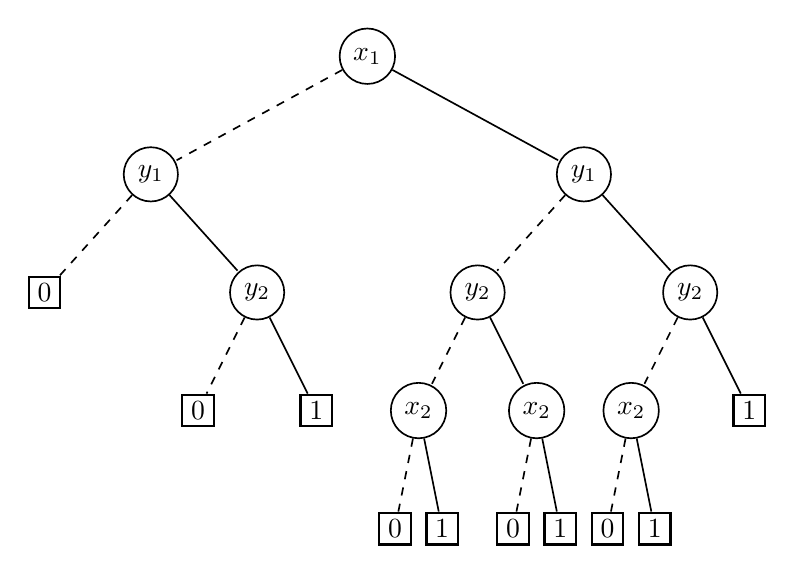
\begin{tikzpicture}[
  level 1/.style={sibling distance=55mm},
  level 2/.style={sibling distance=27mm},
  level 3/.style={sibling distance=15mm},
  level 4/.style={sibling distance=6mm},
  -,>=stealth',shorten >=0.5pt,auto,node distance=1cm,semithick,term/.style={draw,rectangle,minimum size=4mm,inner sep=0pt,outer sep=0pt,solid,thick}]
      \tikzstyle{every state}=[fill=white,draw=black,text=black,inner sep=3pt,minimum size=4pt,solid]
      
      
     \node [state] (a){$x_1$}
     child[dashed]{
      node [state] (b){$y_1$}
      child[dashed]{
	node [term] (c){$0$}
      }
      child[solid]{
	node [state] (c){$y_2$}
	child[dashed]{
	  node [term] (d){$0$}	  
	}
	child[solid]{
	  node [term] (d){$1$}
	}
      }
     }
     child[solid]{
      node [state] (b){$y_1$}
      child[dashed]{
	node [state] (c){$y_2$}
	child[dashed]{
	  node [state] (d){$x_2$}
	  child[dashed]{
	    node [term] (e){$0$}	    
	  }
	  child[solid]{
	    node [term] (e){$1$}	    
	  }
	}
	child[solid]{
	  node [state] (d){$x_2$}
	  child[dashed]{
	    node [term] (e){$0$}	    
	  }
	  child[solid]{
	    node [term] (e){$1$}	    
	  }
	}
      }
      child[solid]{
	node [state] (c){$y_2$}
	child[dashed]{
	  node [state] (d){$x_2$}
	  child[dashed]{
	    node [term] (e){$0$}	    
	  }
	  child[solid]{
	    node [term] (e){$1$}	    
	  }
	}
	child[solid]{
	  node [term] (d){$1$}	  
	}
      }
     };
 
  \end{tikzpicture}
  \caption{Using C2 we remove the redundant tests and eliminate the nodes leading to them. We derive the above reduced diagram.}

\end{figure}

\begin{figure}[H]
  \label{fig:robdd23}
  \centering
  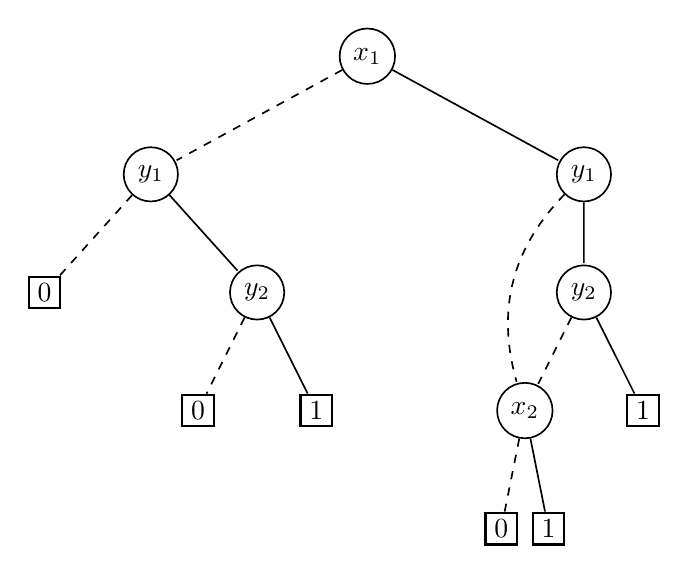
\begin{tikzpicture}[
  level 1/.style={sibling distance=55mm},
  level 2/.style={sibling distance=27mm},
  level 3/.style={sibling distance=15mm},
  level 4/.style={sibling distance=6mm},
  -,>=stealth',shorten >=0.5pt,auto,node distance=1cm,semithick,term/.style={draw,rectangle,minimum size=4mm,inner sep=0pt,outer sep=0pt,solid,thick}]
      \tikzstyle{every state}=[fill=white,draw=black,text=black,inner sep=3pt,minimum size=4pt,solid]
      
      
     \node [state] (A){$x_1$}
     child[dashed]{
      node [state] (B1){$y_1$}
      child[dashed]{
	node [term] (C1){$0$}
      }
      child[solid]{
	node [state] (C2){$y_2$}
	child[dashed]{
	  node [term] (D1){$0$}	  
	}
	child[solid]{
	  node [term] (D2){$1$}
	}
      }
     }
     child[solid]{
      node [state] (B2){$y_1$}
      child[solid]{
	node [state] (C3){$y_2$}
	child[dashed]{
	  node [state] (D5){$x_2$}
	  child[dashed]{
	    node [term] (E5){$0$}	    
	  }
	  child[solid]{
	    node [term] (E6){$1$}	    
	  }
	}
	child[solid]{
	  node [term] (D6){$1$}	  
	}
      }
     };
     
       \path 
	(B2) edge[dashed,bend right]			node{} (D5);

 
  \end{tikzpicture}
  \caption{Using C3 we remove the duplicate non-terminals, redirect the incoming edges and derive the above reduced diagram.}

\end{figure}
\begin{figure}[H]
  \label{fig:robdd24}
  \centering
  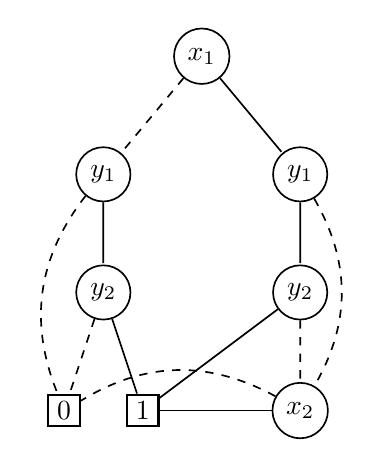
\begin{tikzpicture}[
  level 1/.style={sibling distance=25mm},
  level 2/.style={sibling distance=27mm},
  level 3/.style={sibling distance=10mm},
  level 4/.style={sibling distance=6mm},
  -,>=stealth',shorten >=0.5pt,auto,node distance=1cm,semithick,term/.style={draw,rectangle,minimum size=4mm,inner sep=0pt,outer sep=0pt,solid,thick}]
      \tikzstyle{every state}=[fill=white,draw=black,text=black,inner sep=3pt,minimum size=4pt,solid]
      
      
     \node [state] (A){$x_1$}
     child[dashed]{
      node [state] (B1){$y_1$}
      child[solid]{
	node [state] (C2){$y_2$}
	child[dashed]{
	  node [term] (D1){$0$}	  
	}
	child[solid]{
	  node [term] (D2){$1$}
	}
      }
     }
     child[solid]{
      node [state] (B2){$y_1$}
      child[solid]{
	node [state] (C3){$y_2$}
	child[dashed]{
	  node [state] (D5){$x_2$}
	  }
      }
     };
     
       \path 
       	(B1) edge[dashed,bend right]			node{} (D1)
       	(C3) edge[right]				node{} (D2)
       	(D5) edge[dashed,bend right]			node{} (D1)
       	(D5) edge[left]				node{} (D2)
	(B2) edge[dashed,bend left]			node{} (D5);

 
  \end{tikzpicture}

\caption{Using C1 we remove all the duplicate terminals. This OBDD cannot be reduced any further so we can now call it the canonical of the previous diagrams.}

\end{figure}

\subsection*{Discuss how ordering impacts ROBDD}
\subsection*{Suggest an algorithm for choosing ordering}

\end{document}
